\section{Problemanalyse und Realisation}
\label{sec:analyseUndRealisation}
\subsection{Problemanalyse}
Hierbei habe ich mich einer Technik bedient in der man versucht sich in eine jeweilige Teilkomponente des Problems hineinzuversetzen und anzugeben f"ur welchen Teilbereich diese Komponente verantwortlich ist. Anschlie"send ist es etwas einfach sowie "ubersichtlicher sich auf die Struktur festzulegen, da man s"amtliche Nomen als Klassen ansehen kann (hier einmal \colorbox{Apricot}{orange} dargestellt). Verben spiegeln die ben"otigten Methoden wieder (hier \colorbox{SpringGreen}{gr"un} dargestellt).

\begin{enumerate}
	\item Benutzer
	\begin{enumerate}
		\item Als \colorbox{Apricot}{Benutzer} möchte ich den aktuellen Spielstand in eine Datei mit Auswahl des Dateinamens \colorbox{SpringGreen}{speichern}. Das Logging wird mit \colorbox{SpringGreen}{gespeichert}.
		\item Als \colorbox{Apricot}{Benutzer} möchte ich eine Datei mit einem Spielstand  \colorbox{SpringGreen}{auswählen} und \colorbox{SpringGreen}{öffnen} können.
		\item Als \colorbox{Apricot}{Benutzer} möchte ich ein \colorbox{Apricot}{Spiel} initialisieren und neu starten.
		\item Als \colorbox{Apricot}{Benutzer} möchte ich ein \colorbox{Apricot}{Spiel} \colorbox{SpringGreen}{beenden} (mit/ohne zu \colorbox{SpringGreen}{speichern}).
		\item Als \colorbox{Apricot}{Benutzer} möchte ich das Laden oder Speichern  \colorbox{SpringGreen}{loggen} k"onnen.
	\end{enumerate}	
	\item Spieler
	\begin{enumerate}
		\item Als \colorbox{Apricot}{Spieler} möchte ich einen \colorbox{Apricot}{Domino} \colorbox{SpringGreen}{auswählen}.
 		\item Als \colorbox{Apricot}{Spieler} möchte ich einen \colorbox{Apricot}{Domino} \colorbox{SpringGreen}{drehen}.
		\item Als \colorbox{Apricot}{Spieler} möchte ich einen \colorbox{Apricot}{Domino} \colorbox{SpringGreen}{setzen}.
		\item Als \colorbox{Apricot}{Spieler} möchte ich das Stadtzentrum \colorbox{SpringGreen}{bewegen}.
		\item Als \colorbox{Apricot}{Spieler} möchte ich meine Aktionen \colorbox{SpringGreen}{loggen}.
	\end{enumerate}
	\item Spiel
	\begin{enumerate}
		\item Als \colorbox{Apricot}{Spiel} möchte ich die \colorbox{Apricot}{Spielfelder} der Spieler \colorbox{SpringGreen}{visualisieren}.
		\item Als \colorbox{Apricot}{Spiel} möchte ich die \colorbox{Apricot}{Auswahlfelder} \colorbox{SpringGreen}{visualisieren}.
		\item Als \colorbox{Apricot}{Spiel} möchte ich den \colorbox{Apricot}{aktuellen Spielstand} der Spieler \colorbox{SpringGreen}{anzeigen}.
		\item Als \colorbox{Apricot}{Spiel} möchte ich den \colorbox{Apricot}{Gewinner} \colorbox{SpringGreen}{anzeigen}
		\item Als \colorbox{Apricot}{Spiel} möchte ich den \colorbox{Apricot}{Gewinner} \colorbox{SpringGreen}{loggen}.
	\end{enumerate}
\end{enumerate}

\newpage
\subsection{Realisationsanalyse}
\paragraph{Grunds"atzlich ben"otigte Datenstrukturen}
Um eine Partie spielen zu k"onnen werden erst einmal Spielsteine ben"otigt. Hierbei wurden diverse Klassen eingef"uhrt die im Kapitel \nameref{par:domino} \ref{par:domino} auf Seite \pageref{par:domino}
genauer beschrieben werden. Letztendich bieten diese allerdings s"amtliche ben"otigte Schnittstellen um einen Domino mit einer bestimmten Aufschrift sowie Position zu versehen. 

Diese Dominos k"onnen auf Spielbrettern positioniert werden. Jeder Spieler besitzt hierbei eins, und die Gui ist in der Lage diese ordnungsgem"a"s darzustellen. 

Um einen Domino w"ahlen zu k"onnen ist es essentiell einen Konstrukt f"ur eine Bank zu implementieren. Ich habe dabei eine Struktur gew"ahlt in der s"amtliche Spieler nicht anhand irgendeines Indices, sondern anhand ihrer Referenz gespeichert werden. Dies erm"oglicht es mit dem R"uckgabewert einer entsprechenden Getter-Methode direkt arbeiten zu k"onnen, ohne Umwege beim Konvertieren nutzen zu m"ussen. 

\paragraph{Benutzerschnittstelle}
Der Punkt Benutzer entspricht in diesem Projekt s"amtlichen Anfragen die ein Benutzer dem Programm stellen kann. Es bietet sich an eine Struktur zu w"ahlen in der eine Klasse oder Schnittstelle als Anlaufstelle dient "uber die s"amtliche Anfragen bearbeitet werden k"onnen. Hierbei ist nur abzuw"agen ob man eventuell die \glqq Antwort\grqq {} des Programms gleich in diese Schnittstelle mit aufnimmt. Dies führt allerdings zu un"ubersichtlichem Code. 

\paragraph{Spielerverhalten}
Der Punkt Spieler beschreibt die wirklichen Spielteilnehmer. Er muss in der Lage sein selbstst"andig oder durch die Interatktion mit der Gui einen Zug vollziehen zu k"onnen. Hierzu geh"ort das auswahlen, drehen und setzen eines Dominos. Es gilt abzuw"ahlen ob dies durch eine gemeinsame Klasse geschehen soll. Ich habe mich allerdings f"ur eine Unterteilung entschieden, da der menschliche Spieler auf die Eingabe des Benutzers reagiert, w"ahrend die Bots diese mehr oder weniger ignorieren und isoliert ihre eigenen Z"uge vollziehen. 

Desweiteren ben"otigt der Spieler ein Spielbrett auf dem er Dominos setzen kann. Man k"onnte das Spielbrett auch der Verwaltung (also der Spiel-Klasse) "ubergeben, dann w"are ein k"unstlicher Spieler aber nicht mehr derartig isoliert wie es in diesem meinem Entwurf der Fall ist.Iindem die k"unstlichen Spieler selbst alle wichtigen Schritte ausf"uhren, ist so m"oglich eine minimale Schnittstelle dem Spiel (der Verwaltung) gegen"uber bereitzustellen. 

Die Kapsellung des Spielerverhaltens erm"oglicht es au"serdem wartbaren Code zu erzeugen. Es ist einfacher Fehler zu beheben oder bestimmte Prozesse auszutauschen ohne das komplette Programm umstrukturieren zu m"ussen. Am wichtigsten hierbei ist die M"oglichkeit der Erweiterbarkeit. Durch die Kapselung ist es m"oglich s"amtliche Schritte eines Spielers polymorph zu gestalten. Jede Spielerart reagiert also anders auf eine Anfrage und es nicht n"otig den Aufruf hierf"ur zu ver"andern. All diese M"oglichkeiten w"urden entfallen, wenn man das Spielverhalten der k"unstlichen Spieler in der Spiel-Klasse aufrufen w"urde.

\paragraph{Spielerinstantiierung}
Um die Bindung zum Spiel so gering wie m"oglich zu halten (wie im letzten Absatz erkl"art). Habe ich versucht auch bei der Instantiierung m"oglichst nachhaltigen Code zu schreiben indem ich eine statische Fabrikmethode verwende um die einzelnen Spieler zu instantiieren. Letztendlich verschiebt man mit solch einer Fabrik lediglich die Instantierung in eine gemeinsame Methode, allerdings muss man im sp"ateren Verlauf der Entwicklung auch nur hier Dinge "andern. Dies ist besonders hilfreich beim hinzuf"ugen weiterer Spielertypen. Die Fabrik-Methode befindet sich in einem Enum namens \emph{Playertypes}. Diese Enum-Werte k"onnen in gewisser Weise aber auch als Platzhalter f"ur die \glqq richtigen\grqq {} Spieler herhalten. Wie das funktioniert wird im folgendem Abschnitt beschrieben. 

\paragraph{Alternative Spielerinitialisierung}
\label{par:alternativeSpielerinitialisierung}
Der Vorgang des Instantiierens in der Fabrik-Methode ist relativ aufwendig. Man h"atte im Prinzip auch komplett auf die Fabrik verzichten k"onnen, auf lange Sicht ist es aber effektiver Sie hier einzuf"uhren da man sonst nur sehr umst"andlich ein Auswahlfeld f"ur m"ogliche Spieler starten kann. Hierzu folgendes Szenario: Es gibt N Spielertypen unter denen der Benutzer seine Gegner w"ahlen kann. Daf"ur gibt es ein eigenes Auswahlfenster, welches vor dem eigentlichen Spiel auftauchen soll (siehe Abbildung \ref{fig:auswahlfenster}, S. \pageref{fig:auswahlfenster}). Der Controller dieses Fensters "ubernimmt somit die Aufgabe der Main-Methode das Spiel zu starten. Diese tut genau dasselbe wie die urspr"ungliche Main-Methode indem Sie das FXML-Dokument aufruft. Der Controller wird dabei automatisch gestartet und die Initialize-Methode der Controller-Klasse des GameFXML-Dokuments durchlaufen. Hierbei habe ich bei meinen "Uberlegungen keinen Weg gefunden Argumente der Initialize-Methode zu "ubergeben, da diese ja das Interface Initializable implementiert und somit die Signatur nicht ver"andert werden kann. Daher gibt es eine eine Methode welche losgel"ost vom Konstruktor das Spiel mit "ubergebenen Spielertypen starten kann. Dieser Ansatz funktioniert soweit und ist in der Main-Klasse als auskommentierter Block mit dem Schl"usselwort \glqq Alternative\grqq {} gekennzeichnet. Falls dieser Block einkommentiert und der Rest der Main-Methode auskommentiert wird, startet ein Auswahlfenster mit einer M"oglichkeiten der Spielerselektierung. Dies ist allerdings noch nicht ausgereift da es lediglich zur Darstellung des Problems dienen soll, sodass bei invalider Selektierung eine Exception geworfen wird. 

Es gibt zwar bereits einen weiteren Spielertypen, dieser ist allerdings lediglich durch den Umstand entstanden, dass ich die Aufgabenstellung zuerst falsch verstanden habe. In der Aufgabenstellung steht, dass der k"unstliche Spieler bei Punktegleichheit mehrerer potentieller Positionen f"ur einen Domino die jenige w"ahlen soll, welche die geringste Anzahl an Einzelzellen produziert. Hierbei habe ich allerdings f"alschlicher Weise angenommen, dass damit einzelne Distrikte gemeint sind. In der Version des Bots, welche sich im endg"ultigem Spiel wiederfindet wurde dies aber behoben und es wird auf die Einzelzellen au"serhalb der Distrikte geachtet. 

\begin{figure}
	\centering
	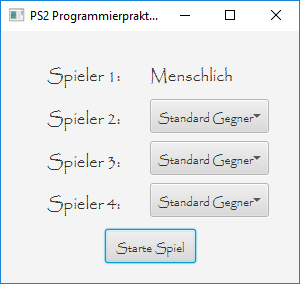
\includegraphics[width=.4\linewidth]{pics/Intro240918}
	\caption[Auswahlfenster]{Auswahlfenster}
	\label{fig:auswahlfenster}
\end{figure}

\paragraph{Spiel}
Dieser Begriff beschreibt koordinierte Abarbeitung der Spielerz"uge. Es wird der Benutzeroberfl"ache mitgeteilt was angezeigt werden soll. Ausserdem werden s"amtliche Stapel von Dominos bereitgestellt die f"ur ein vollwertiges Spiel genutzt werden sollen (Beutel, B"anke). Alle ben"otigten Dateioperationen werden hier eingeleitet aber nicht direkt in dieser Klasse bearbeitet. Durch das ganze Exceptionhandling wird es ziemlich un"ubersichtlich die gesamte Funktionalit"at in das Spiel zu verlagern, da dieses in erster Linie f"ur die "ubergeordnete Organisation des ganzen Programms gedacht ist. 

\paragraph{Log}
Da man vermehrt, und vor allem an vielen verschiedenen Stellen im Code, eine neue Zeile in die Logdatei schreiben, beziehungsweise auf der Konsole ausgeben m"ochte, bietet sich f"ur die Implementierung des Loggers das \emph{Singleton-Muster} an. Dieses Muster verwaltet eine einzige globale Instanz auf die immer wieder zugegriffen wird. Das Muster eignet sich besonders gut f"ur das Loggen von Daten, da man alles in die selbe Datei schreiben m"ochte und diese nicht jedesmal neu \emph{suchen / anlegen} muss. Im Logger kann man zum Beispiel einfach ein entsprechendes Feld verwalten. 

\paragraph{Speichern und Laden}
Auch beim Speichern und Laden wird in diesem Entwurf ein \emph{Singleton-Muster} verwendet. Da man beim Speichern jeweils den Dateipfad, nach erstmaliger Eingabe, nicht erneut eingeben m"ochte wenn dies nicht unbedingt erforderlich ist (siehe Abschnitt 
\emph{Speichern als} gegen"uber \emph{Speichern}, \ref{spar:anleitung_speichern} auf Seite \pageref{spar:anleitung_speichern}). Und auch das Speichern und Laden erstreckt sich vermehrt "uber das gesamte Projekt. Alternativ k"onnte man auch ein klassische Klasse verwenden, wegen den genannten Punkten empfiehlt sich aber gerade f"ur diese beiden Anwendungsf"alle das Muster. F"ur eine genauere Beschreibung des Musters siehe \ref{par:singletonMuster} \nameref{par:singletonMuster} auf Seite \pageref{par:singletonMuster}. 
